% UQ Gemini theme
% See: https://github.com/alfurka/gemini-uq
% Forked from
% https://rev.cs.uchicago.edu/k4rtik/gemini-uccs
% which is forked from
% https://github.com/anishathalye/gemini


\documentclass[final]{beamer}

% ====================
% Packages
% ====================

\usepackage[T1]{fontenc}
\usepackage{lmodern}
\usepackage[size=custom,width=100,height=75,scale=1.0]{beamerposter}
\usetheme{gemini}
\usecolortheme{uchicago}
\usepackage{graphicx}
\usepackage{booktabs}
\usepackage{tikz}
\usepackage{pgfplots}
\pgfplotsset{compat=1.17}

% ====================
% Lengths
% ====================

% If you have N columns, choose \sepwidth and \colwidth such that
% (N+1)*\sepwidth + N*\colwidth = \paperwidth
\newlength{\sepwidth}
\newlength{\colwidth}
\setlength{\sepwidth}{0.025\paperwidth}
\setlength{\colwidth}{0.3\paperwidth}

\newcommand{\separatorcolumn}{\begin{column}{\sepwidth}\end{column}}

% ====================
% Title
% ====================

\title{\href{https://dl.acm.org/doi/10.1145/2911451.2911537}{Learning to Rank with Selection Bias in Personal Search}}

\author{Xuanhui Wang \inst{1} \and Michael Bendersky \inst{1}}

\institute[shortinst]{\inst{1} Google Inc.}

% ====================
% Footer (optional)
% ====================

\footercontent{
  \href{https://github.com/AliannejadiPourya}{Github} \hfill
  Pourya Aliannejadi \hfill
  \href{mailto:alian.pourya@gmail.com}{alian.pourya@gmail.com}}
% (can be left out to remove footer)

% ====================
% Logo (optional)
% ====================

% use this to include logos on the left and/or right side of the header:
% \logoright{\includegraphics[height=7cm]{logo1.pdf}}
% \logoleft{\includegraphics[height=7cm]{logo2.pdf}}

% ====================
% Body
% ====================

\begin{document}
\addtobeamertemplate{headline}{}
{
    \begin{tikzpicture}[remember picture,overlay]
      \node [anchor=north west, inner sep=3cm] at ([xshift=0.0cm,yshift=1.0cm]current page.north west)
      {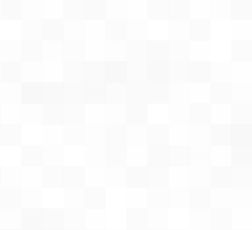
\includegraphics[height=5.0cm]{logos/Logo-Left.png}}; % also try shield-white.eps
      \node [anchor=north east, inner sep=3cm] at ([xshift=2.0cm,yshift=2.0cm]current page.north east)
      {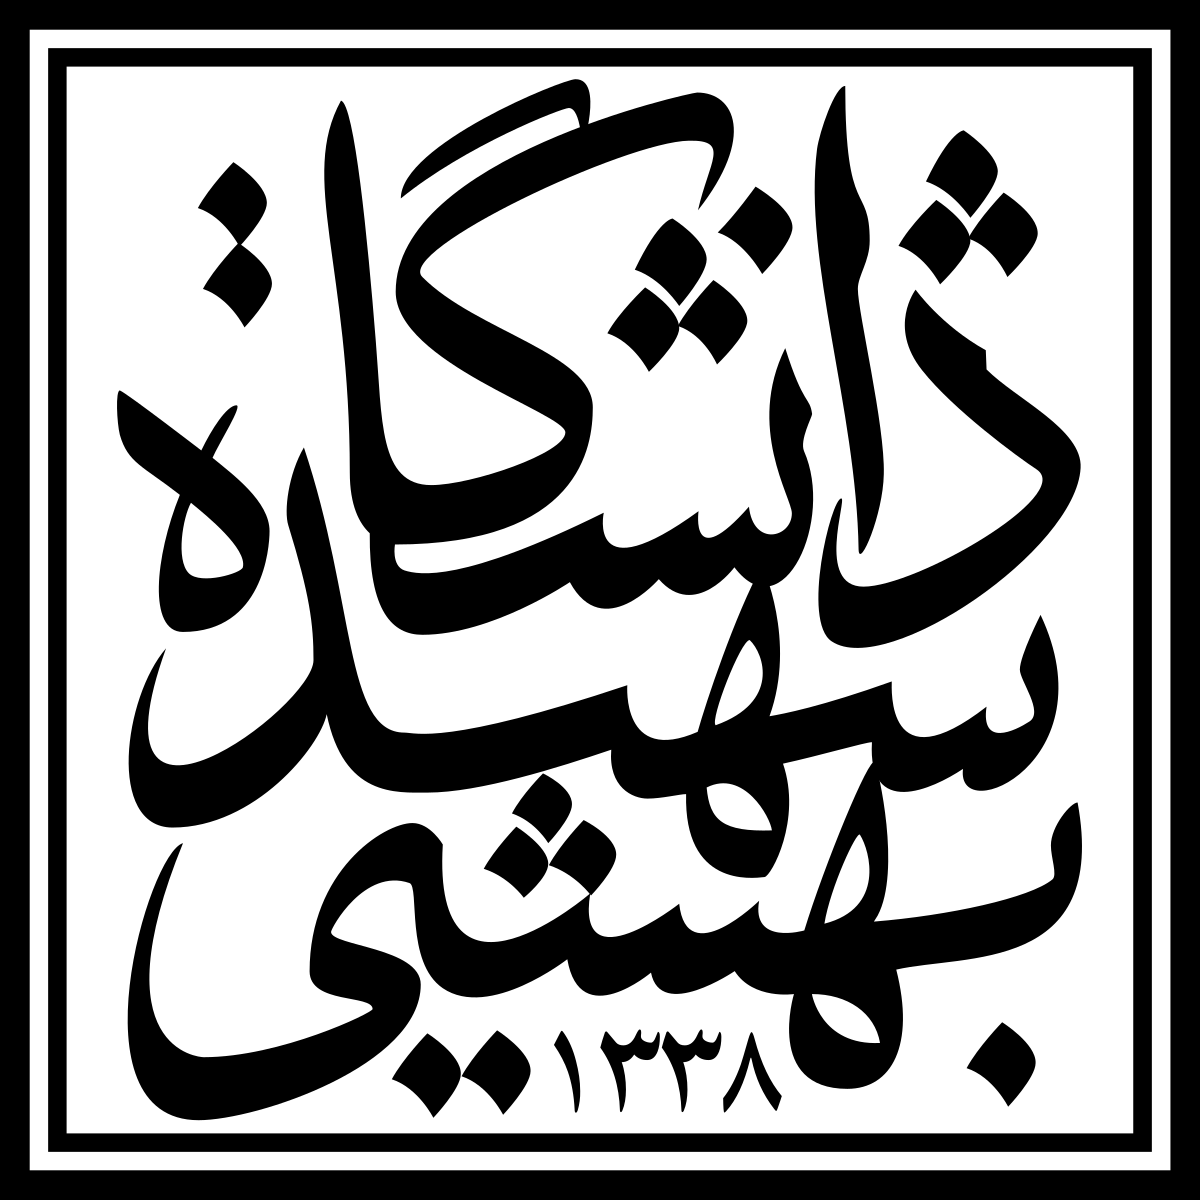
\includegraphics[height=7.0cm]{logos/Logo-Right.png}};
    \end{tikzpicture}
}

\begin{frame}[t]
\begin{columns}[t]
\separatorcolumn

\begin{column}{\colwidth}
  \begin{block}{Research Gap}
    The paper addresses the research gap in effectively leveraging sparse click-through data for learning-to-rank in personal search. Existing click models typically require large quantities of clicks per query-document pair, which is \textbf{not feasible in personal search} due to personalized corpora and information needs. Furthermore, obtaining explicit relevance judgments in personal search is difficult due to privacy and the dynamic nature of personal data. The paper also identifies a novel selection bias problem in this context, where queries with clicks are under-sampled in a biased manner, affecting the learning process.
  \end{block}

  \begin{block}{Main Contributions}
    \begin{itemize}
      \item Introduces the \textbf{selection bias problem} in learning-to-rank for personal search.
      \item Proposes several \textbf{bias estimation models}, including a \textbf{query-dependent (generalized) model} that does not require large amounts of click data.
      \item Presents a novel \textbf{unbiased offline evaluation methodology} based on randomized result sets.
      \item Validates the models through large-scale \textbf{offline and online experiments} on a real personal search engine.
    \end{itemize}
  \end{block}

  \begin{block}{Method Overview}
	The key method used is \textbf{inverse propensity weighting} to address the selection bias. The paper estimates the propensity score (the probability of a query appearing in the clicked data) and uses its inverse to weight the loss function during learning-to-rank. Different models for estimating these inverse propensity weights are proposed: a \textbf{global bias model} based on position, a \textbf{segmented bias model} based on query segments (email labels), and a \textbf{generalized bias model} using \textbf{multi-class logistic regression with query-dependent features} to predict position bias. \textbf{Result randomization} is employed to collect unbiased data for bias estimation.
    \begin{figure}
      \centering
      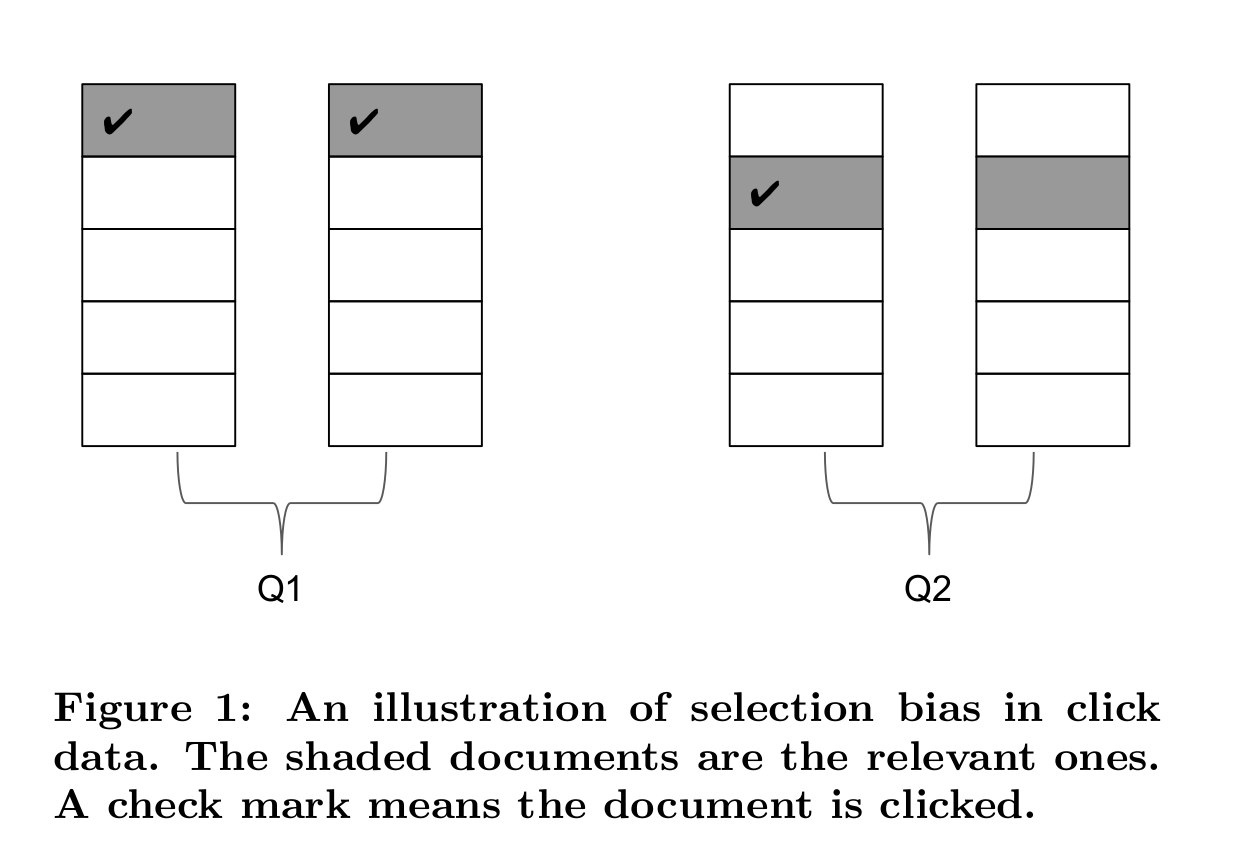
\includegraphics[width=0.9\linewidth]{fig 1.png}
      \caption{Selection bias in click
      	data.}
    \end{figure}
  \end{block}
\end{column}

\separatorcolumn

\begin{column}{\colwidth}

  \begin{block}{Key Findings}
    \begin{itemize}
      \item Accounting for \textbf{query-dependent selection bias} in learning-to-rank significantly improves search effectiveness (MRR and CTR) in online experiments with a large-scale personal search engine compared to a baseline without bias correction.
      \item \textbf{More fine-grained bias models} (segmented and generalized) lead to further improvements over a global bias model, with the segmented model showing significant improvement over the global model in online A/B testing.
      \item The proposed \textbf{unbiased offline evaluator provides a sound methodology} for evaluating ranking functions on randomized data, addressing the limitations of standard offline metrics in the presence of selection bias.
    \end{itemize}
  \end{block}

  \begin{block}{Strengths and Weaknesses}
    \textbf{Strengths}:
    \begin{itemize}
      \item \textbf{First} to comprehensively study selection bias in personal search ranking.
      \item Uses \textbf{real-world large-scale deployment} with randomized experiments.
      \item Develops a novel offline evaluation strategy that \textbf{overcomes bias} from using regular click data.
    \end{itemize}
    \textbf{Weaknesses}:
    \begin{itemize}
      \item The offline evaluation showed \textbf{no statistically significant difference} between the segmented and generalized models, potentially due to the limited size of the evaluation data. 
      \item Evaluations limited to \textbf{single-click queries} and \textbf{personal search scenarios}—not generalized to multi-click or broader search settings.
    \end{itemize}
  \end{block}

  \begin{block}{Future Directions}
    \begin{itemize}
      \item Evaluating the applicability of these methods to \textbf{web search}.
      \item Extending the framework to handle \textbf{multiple clicks per query}.
      \item Investigating effective features for \textbf{bias estimation in different application domains}.
      \item Exploring \textbf{cheaper and less intrusive} methods for collecting randomized data.
      \item Improving the \textbf{data utilization} of the unbiased offline evaluator.
    \end{itemize}
  \end{block}
\end{column}


\separatorcolumn
\begin{column}{\colwidth}
  \begin{block}{Core Equation}
    \textbf{Inverse Propensity Weighting for Empirical Loss}:
    \[
    L_S(f) = \frac{1}{|S|} \sum_{Q \in S} \frac{P(Q)}{\hat{P}(Q)} \cdot l(Q, f) = \frac{1}{|S|} \sum_{Q \in S} w_Q \cdot l(Q, f)
    \]
    
    \textit{Where \({\hat{P}(Q)}\) is known as the propensity score of \(Q\).}
  \end{block}

  \begin{block}{List of position bias prediction methods}
	   \begin{figure}
	\centering
	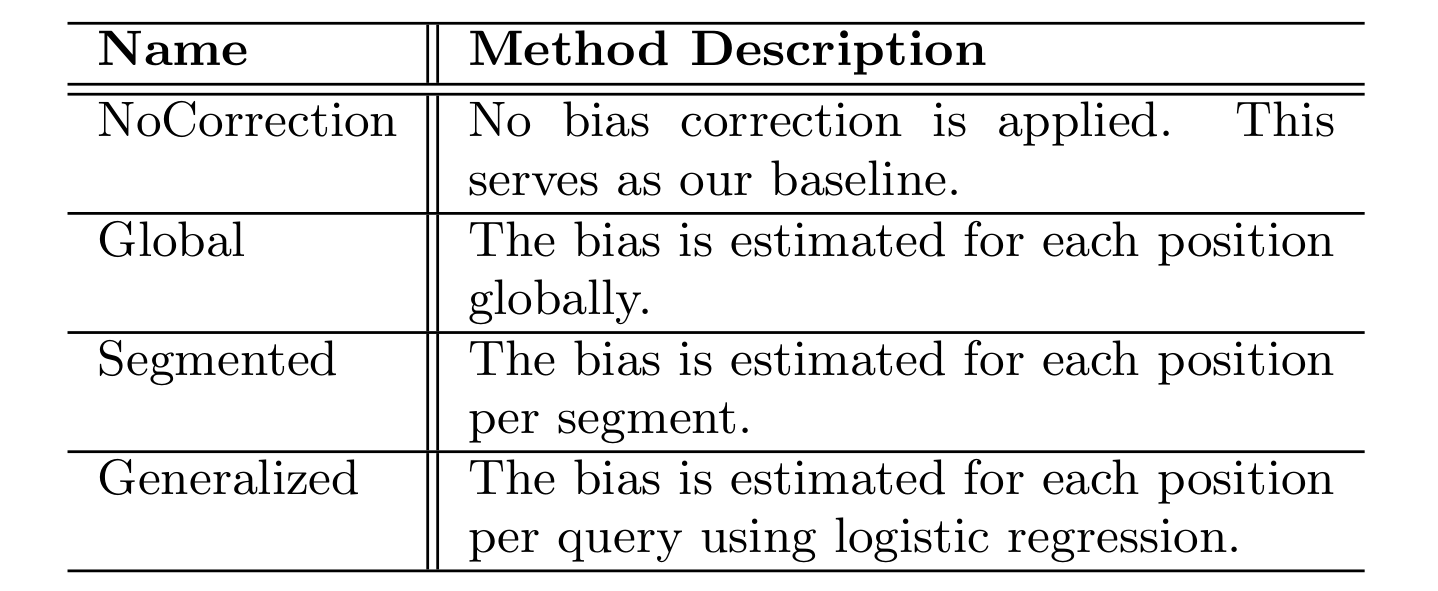
\includegraphics[width=0.9\linewidth]{fig 2.png}
	\end{figure}
  \end{block}


	\begin{block}{Example}
	    \begin{figure}
		\centering
		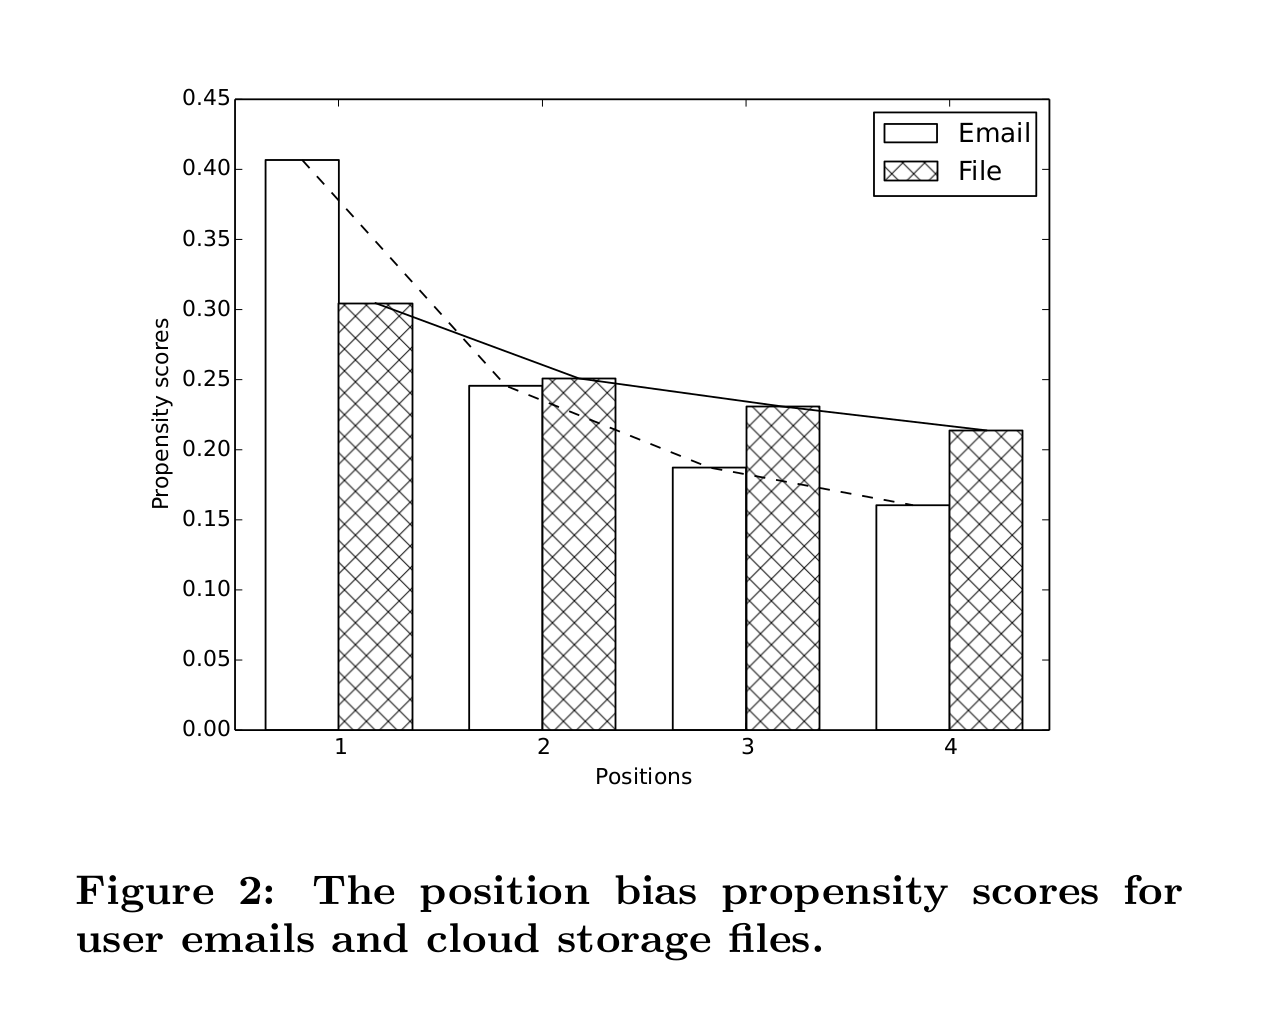
\includegraphics[width=0.9\linewidth]{fig 3.png}
		\end{figure}
	\end{block}
	

\end{column}

\separatorcolumn
\end{columns}
\end{frame}

\end{document}
